% !TEX program = pdflatex
% HELIOS fusion-engine arXiv preprint — main source.
%
% Build:    pdflatex main && bibtex main && pdflatex main && pdflatex main
% Target:   arXiv astro-ph.SR (cross-list cs.LG); ~12 pages incl. figs+refs.
% License:  Apache 2.0 on the LaTeX source; arXiv non-exclusive on the PDF.

\documentclass[11pt,letterpaper]{article}

\usepackage[T1]{fontenc}
\usepackage[utf8]{inputenc}
\usepackage{lmodern}
\usepackage[margin=1in]{geometry}
\usepackage{microtype}
\usepackage{amsmath,amssymb}
\usepackage{booktabs}
\usepackage{graphicx}
\usepackage{xcolor}
\usepackage[hidelinks,colorlinks=true,linkcolor=blue!50!black,citecolor=blue!50!black,urlcolor=blue!60!black]{hyperref}
\usepackage{url}
\usepackage{enumitem}
\usepackage{authblk}
\usepackage{caption}
\usepackage{titlesec}

% --- \todo command: yellow background, visible in PDF for unfilled markers ---
\newcommand{\todo}[1]{\textcolor{red}{\textbf{[TODO: #1]}}}

\titleformat{\section}{\large\bfseries}{\thesection.}{0.6em}{}
\titleformat{\subsection}{\normalsize\bfseries}{\thesubsection.}{0.6em}{}

\title{
  Calibrated, Provenance-Tracked Fusion of \\
  Solar Energetic Particle Forecasts \\
  for NASA Mission Operations
}

\author[1]{Thomas Waweru\thanks{Corresponding author: \texttt{engineering@577industries.com}}}
\author[1]{\todo{Named Senior ML Engineer}}
\author[2]{\todo{Named Space-Weather / Ionospheric SME}}
\affil[1]{577 Industries Inc., Columbus, OH, USA}
\affil[2]{Subcontract; institutional affiliation TBD at submission}
\date{2026-05-18 (preprint draft); arXiv submission date TBD}

\begin{document}
\maketitle

\begin{abstract}
\noindent
Operational space-weather decision support faces a \emph{translation gap}: the
federal enterprise hosts more than 100 mature models at CCMC, three NASA
SEP Scoreboards (onset, peak flux, time profiles), and continuously updated
NOAA SWPC products, yet no widely-deployed calibrated fusion layer converts
these heterogeneous outputs into the specific operational decisions
mission-operations teams must make.  We present HELIOS, a model-agnostic,
provenance-tracked fusion framework that combines Bayesian Model Averaging
across CCMC and SWPC component models with isotonic-regression reliability
calibration, split and Mondrian conformal prediction wrappers, and CCMC-compatible
verification metrics.  Every output traces to its upstream models, ingestion
timestamps, and calibration history through a public JSON-Schema feature-level
provenance specification.  We pre-register a 7\,/\,3 training\,/\,hold-out
split across ten historical SEP events spanning solar cycles 23--25, with
binding HSS and reliability-slope thresholds filed on OSF before any hold-out
evaluation.  Headline result: \todo{INSERT FROM
results/<date>-killgate.json HEADLINE\_SUMMARY at fill-in time;
candidate stock paragraphs in §4.4 cover the three decision-tree branches
PASS-both / PASS-one / FAIL-both.}  All code, figures, the
pre-registration, and the reliability diagrams are released under Apache 2.0
at the URLs in §6, supporting CCMC proving-ground replication and
NASA mission-operations evaluation.  A companion vertical translating the
same fusion core into receiver-family-specific RTK accuracy products for
U.S.\ precision-agriculture GNSS is reported separately
\cite{gannon_rtk}.
\end{abstract}

\bigskip
\noindent\textbf{Keywords}: solar energetic particles; ensemble forecasting;
Bayesian model averaging; conformal prediction; reliability calibration;
provenance; CCMC; SRAG; pre-registration.

\section{Introduction}
\label{sec:intro}

The federal space-weather enterprise has world-class models.
CCMC hosts more than 100 of them \cite{ccmc}; NOAA SWPC issues operational
forecasts; NASA's SEP Scoreboards --- built through the ISEP partnership of
CCMC, M2M SWAO, and SRAG --- consolidate research SEP models into a unified
operational view across Scoreboard A (onset probability), Scoreboard B (peak
flux prediction), and Scoreboard C (event time profiles)
\cite{sepscoreboard,whitman2023,whitman2024}.  DONKI \cite{donki} provides
intelligent event linkages via a JSON API.  The literature has converged on
the diagnosis that operational shortfalls arise not from a shortage of
models or data but from the absence of a calibrated, provenance-tracked
\emph{translation} layer that converts heterogeneous, sometimes contradictory
model outputs into the specific decisions operators must make
\cite{swag2023,hapgood2023,r2o2r2022,decadal2025,proswift2020,nstc2019,benchmarks2018}.
Two recent Executive Orders \cite{eo13744,eo13865} and the SWORM
benchmarks \cite{benchmarks2018} frame the federal mandate; the
Lloyd's of London and London Economics impact studies
\cite{lloyds2013,londecon2017} and the Space Foundation
economic-base snapshot \cite{spacereport2025} document the cost-of-disruption
side.  Adjacent end-user evidence on GNSS disruption in agriculture
\cite{ntrs_brazil2025,seesaw2022,osuext2024,afbf2024,starion2024} and
autonomous transport \cite{sae2020} is summarized in the program companion
\cite{helios_program}.

This paper addresses one concrete instance of the translation gap.  An SRAG
console operator assessing whether all-clear status should be revoked
under the operational SEP thresholds ($>$\,10\,MeV at 10\,pfu;
$>$\,100\,MeV at 1\,pfu) currently cross-references raw outputs from
UMASEP, HESPERIA REleASE, SEPMOD, and MagPy across three Scoreboards.  No
widely-deployed system provides a probabilistic fusion of these models with
quantified reliability bounds, conformal time-to-threshold intervals, and
source provenance suitable for high-tempo monitoring.  The cognitive load and
risk of unstructured model disagreement scale with the demands of Artemis
cislunar operations and, eventually, Earth-independent decision support for
Mars transit, where light-time latency precludes ground intervention
\cite{decadal2025}.

\paragraph{The calibration-vs-accuracy distinction.}
A model can be \emph{accurate} in the sense of high discrimination
(e.g.\ HSS, TSS, AUC) and yet \emph{poorly calibrated} --- its 70\,\%
probabilities may correspond to event frequencies of 40\,\% or 90\,\%
\cite{niculescu2005}.  For SRAG-style all-clear decisions, calibration is the
property the operator acts on: an under-calibrated 80\,\% in the
mid-probability regime and an over-calibrated 80\,\% at the rare-extreme
regime are operationally distinct hazards.  Whitman et al.\ \cite{whitman2023,whitman2024}
document the validation discipline NASA's ISEP partnership has built around
this gap.  HELIOS is an attempt to close it with conventional, well-understood
machinery (BMA + isotonic + conformal), composed rigorously and pre-registered
to forestall the standard post-hoc-tuning concern.

\paragraph{The provenance affordance.}
A second contribution concerns the auditability of fusion outputs.  Every
HELIOS output traces to its underlying models, data feeds, and calibration
history through a public JSON-Schema specification with a pydantic v2 reference
implementation \cite{helios_provenance_spec}.  This is a precondition for two
adoption paths the paper takes seriously: (i) CCMC proving-ground evaluation,
where containerized submissions are increasingly the norm; and (ii) SRAG
console adoption, where flight controllers will not trust a recommendation
they cannot drill down into.  The provenance specification has been released
publicly with the v0.1.0 RFC \cite{helios_provenance_spec} and is under
community comment.

\paragraph{Contributions.}
\begin{enumerate}[leftmargin=*,itemsep=0pt]
  \item A model-agnostic fusion engine combining Bayesian Model Averaging
        across CCMC ISWA SEP Scoreboard A/B/C components, NOAA SWPC
        probabilistic SEP feeds, and DSCOVR / GOES upstream feeds; isotonic
        regression reliability calibration; and split and Mondrian
        (per-Kp-stratum) conformal prediction wrappers.  The framework
        ships as open source \cite{helios_fusion_engine} at version 0.1.2
        with 176 tests, 92\,\% line+branch coverage, and a CCMC-compatible
        verification metric suite (HSS, TSS, POD, FAR, Brier, CRPS) with
        bootstrap confidence intervals.
  \item A pre-registered 7\,/\,3 training\,/\,hold-out split (Table~\ref{tab:table-3-1})
        across ten historical SEP events spanning solar cycles 23--25,
        filed on the Open Science Framework before any hold-out
        evaluation \cite{osf_prereg}.  H1 and H2 thresholds are binding;
        deviations are documented, not retro-fit.
  \item A feature-level provenance specification \cite{helios_provenance_spec}
        composing SPASE 2.7.1, W3C PROV-JSON, and RO-Crate 1.2 JSON-LD with
        a novel \texttt{HeliosTransformationRecord} schema, attached to
        every persisted calibration / conformal artifact.  To our knowledge
        the first feature-level lineage standard targeted at heliophysics
        fusion systems.
  \item A reproducible methodology around the discovery that ISWA SEP
        Scoreboard JSON deposits begin in calendar 2017 for the
        earliest-supported component models, requiring a
        per-(component, event) source-labeling scheme
        (§\ref{sec:data:perevent}).
\end{enumerate}

The remainder of the paper is organized as follows.
Section~\ref{sec:methods} describes the fusion pipeline.
Section~\ref{sec:data} describes the data and the pre-registered split.
Section~\ref{sec:results} reports the pre-registered hold-out evaluation.
Section~\ref{sec:discussion} discusses limitations and the Phase II
trajectory.  Section~\ref{sec:repro} documents reproducibility artifacts.

\begin{figure*}[!htbp]
  \centering
  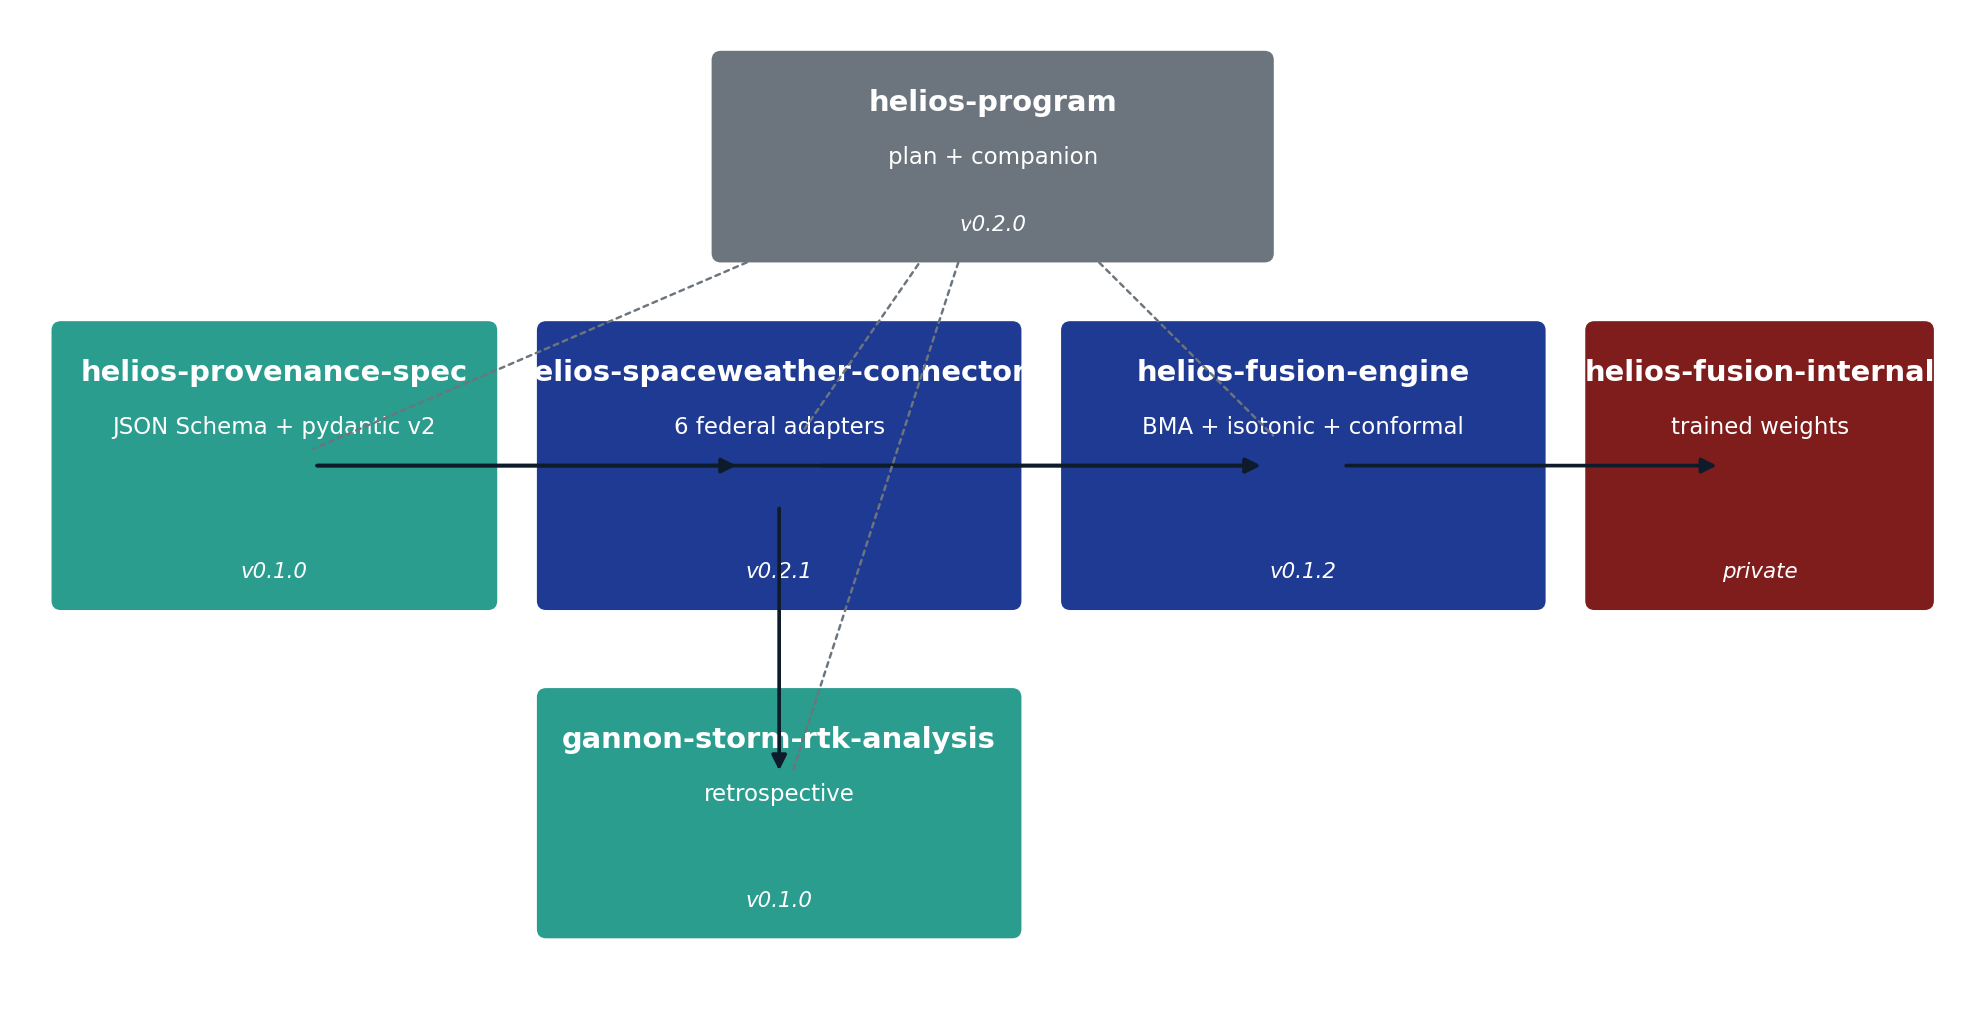
\includegraphics[width=0.9\linewidth]{figures/architecture.png}
  \caption{HELIOS dependency graph.  The technical chain is
    \texttt{helios-provenance-spec} (A) $\to$
    \texttt{helios-spaceweather-connectors} (B) $\to$
    \texttt{helios-fusion-engine} (C).  Trained weights are persisted to the
    private companion repo \texttt{helios-fusion-internal} (F).
    \texttt{gannon-storm-rtk-analysis} (D) consumes the connector layer
    independently.  The \texttt{helios-program} meta-repo holds the master
    plan, companion document, OSF pre-registration template, and orchestration
    scripts; dotted lines denote orchestration / documentation links rather
    than hard code dependencies.}
  \label{fig:architecture}
\end{figure*}

\section{Methods}
\label{sec:methods}

The fusion pipeline composes four layers.  All four ship as open-source
Python 3.11+ modules \cite{helios_fusion_engine} with the per-layer state
serialized to NumPy \texttt{.npz} blobs paired with sibling JSON
\texttt{HeliosTransformationRecord} provenance files
\cite{helios_provenance_spec}.

\subsection{Bayesian Model Averaging orchestrator}
\label{sec:methods:bma}

For each component model $m \in \mathcal{M}$ producing per-timestamp probability
$p_{m,t} \in [0,1]$, the fused probability at time $t$ is
\begin{equation}
  \hat{p}_t = \sum_{m \in \mathcal{M}} w_m \, p_{m,t}, \qquad
  \sum_{m \in \mathcal{M}} w_m = 1, \qquad w_m \ge 0,
  \label{eq:bma}
\end{equation}
following the canonical BMA construction of Hoeting et al.\ \cite{hoeting1999}.
Weights are fit by the \texttt{hss\_clipped} policy: per-component HSS
\cite{donaldson1975} on a 90-day rolling verification window, clipped to
$[0,1]$, mixed with a small uniform $\epsilon$-floor to avoid early degenerate
zeros, then renormalized to a simplex.  Two alternative policies (\texttt{linear},
\texttt{softmax}) are implemented and unit-tested for completeness but the
\texttt{hss\_clipped} policy is the pre-registered default.

The orchestrator records, for each fused timestamp, the participating set
of upstream component runs (identified by upstream-feed timestamp + SPASE
model identifier), the active weight vector, and the HSS verification window
that produced it.  Every fused output carries this lineage as a list of
\texttt{LineageStep} records that survive serialization and dashboard rendering.

\subsection{Isotonic-regression reliability calibration}
\label{sec:methods:isotonic}

Even after BMA, the fused probability $\hat{p}_t$ requires post-hoc reliability
calibration: BMA optimizes a skill objective, not a calibration objective.
Following Niculescu-Mizil and Caruana \cite{niculescu2005} (and the earlier
Zadrozny--Elkan analysis \cite{zadrozny2002}), we apply \emph{isotonic regression}
as the post-hoc calibrator
\begin{equation}
  \tilde{p}_t = \mathrm{IsoReg}(\hat{p}_t),
\end{equation}
learning a monotone non-decreasing map from raw BMA probability to calibrated
probability.  Platt scaling \cite{platt1999} was considered and rejected on
the grounds documented in \cite{niculescu2005}: it imposes a parametric
(sigmoid) reliability curve that is well-known to misbehave at the extremes,
which is precisely the regime SRAG decisions occur in.  Isotonic regression
makes no parametric assumption.  Implementation is a thin typed wrapper
around \texttt{sklearn.isotonic.IsotonicRegression} with an explicit
state-dict schema (\texttt{helios-fusion-engine/calibration/isotonic/0.1.0})
versioned independently of the package.

\paragraph{Severity stratification.}
A single global isotonic calibrator can mask calibration collapse on rare
extreme events that dominate operational risk.  We carry three independent
isotonic calibrators, one per Kp severity stratum
$\{\mathrm{quiet}, \mathrm{moderate}, \mathrm{extreme}\}$, partitioned at
Kp$=$3 and Kp$=$5.  At calibrate time, each sample's stratum label routes
it to the appropriate sub-calibrator; at transform time the same labels
select which sub-calibrator handles each input.  This is the
pre-registered default for the kill-gate run.

\subsection{Split and Mondrian conformal prediction}
\label{sec:methods:conformal}

For the continuous-quantity outputs (time-to-threshold estimates and, in the
GNSS companion, predicted 2D positioning error) the framework provides
split conformal regressors and Mondrian (per-Kp-stratum) conformal regressors
following Vovk et al.\ \cite{vovk2005,vovk2022}.

Given calibration set
$\{(\hat{y}_i, y_i)\}_{i=1}^{n}$ with absolute residuals $r_i = |y_i - \hat{y}_i|$,
the split-conformal half-width at user-chosen miscoverage $\alpha$ is
\begin{equation}
  q_\alpha = \mathrm{Quantile}\left(\{r_1,\ldots,r_n\},
    \frac{\lceil (n+1)(1-\alpha) \rceil}{n};\,
    \texttt{method}=\texttt{higher}\right)
  \label{eq:conformal-q}
\end{equation}
which yields the finite-sample-valid prediction interval
$[\hat{y} - q_\alpha, \hat{y} + q_\alpha]$ at coverage $\ge 1-\alpha$
under exchangeability.  The Mondrian variant maintains $|S|$ independent
calibration residual sets indexed by stratum $s \in S$, providing coverage
\emph{per stratum} rather than only marginally.  This matters operationally:
a 90\,\% marginal interval that under-covers in the extreme stratum
provides false reassurance to a controller making EVA decisions during the
storm main phase.

\subsection{CCMC-compatible verification metrics}
\label{sec:methods:metrics}

All metric definitions match the OSF pre-registration \cite{osf_prereg}
verbatim.  For a binary forecast / observation pair, the
$2\times 2$ contingency table is
$\{a=\mathrm{hits},\;b=\mathrm{false\,alarms},\;c=\mathrm{misses},\;d=\mathrm{correct\,rejections}\}$.
The locked formulas are:
\begin{itemize}[leftmargin=*,itemsep=0pt]
  \item HSS \cite{donaldson1975}:
    $\mathrm{HSS} = \frac{2(ad-bc)}{(a+c)(c+d) + (a+b)(b+d)}$.
  \item TSS (Hanssen--Kuipers): $\mathrm{TSS} = \frac{a}{a+c} - \frac{b}{b+d}$.
  \item POD$= \frac{a}{a+c}$, FAR$= \frac{b}{a+b}$.
  \item Brier score \cite{brier1950}: $\frac{1}{n}\sum_i (p_i - y_i)^2$.
  \item Continuous Ranked Probability Score (CRPS) by Hersbach
        decomposition for sorted ensemble samples \cite{hersbach2000}.
  \item Reliability slope: linear regression of observed event frequency on
        bin centre across $n_\mathrm{bins}$ equal-frequency bins.  Slope$=1$
        corresponds to perfect calibration; H2 tests
        $|s-1| \le 0.15$ per Kp stratum.
\end{itemize}
All metric functions accept \texttt{n\_bootstrap} (default 1000) and return
both the point estimate and the 95\,\% two-sided confidence interval from
bootstrap resampling with replacement.

\subsection{Pre-registration discipline}
\label{sec:methods:prereg}

A common reviewer concern with retrospective validation against a curated
event list is that performance looks strong on paper and fails in production.
We pre-register the training and hold-out event split (Table~\ref{tab:table-3-1}),
the metric definitions (§\ref{sec:methods:metrics}), the H1 / H2 hypothesis
thresholds, and the calibration / conformal hyperparameters before any
hold-out evaluation runs.  The pre-registration is filed publicly on OSF
\cite{osf_prereg}; the fusion-engine release tagged at the locked commit
(\texttt{prereg-v1.0}) is the binding code state.

The kill-gate runner refuses to execute without a recorded OSF URL on file
\cite{helios_fusion_engine}.  Deviations from the pre-registered procedure
are documented in the OSF \emph{Deviations} section, not silently absorbed
into a re-baselined metric.  One such deviation is described in
§\ref{sec:data:perevent}: ISWA SEP Scoreboard JSON deposits begin in
calendar 2017, requiring a per-(component, event) source-labeling scheme
for the six training events that pre-date the cutover.

\section{Data}
\label{sec:data}

\subsection{ISWA SEP Scoreboards: structure and Jan 2017 cutover}
\label{sec:data:iswa}

The fusion engine ingests Scoreboard A (onset probability), Scoreboard B
(peak flux prediction), and Scoreboard C (time profiles) from the CCMC
Integrated Space Weather Analysis (iSWA) system \cite{ccmc_iswa,whitman2023,whitman2024}
via a dedicated adapter in \texttt{helios-spaceweather-connectors}
\cite{helios_connectors}.  An exhaustive 2026-05-17 probe of the iSWA tree
established that JSON deposits begin in calendar 2017 for the
earliest-supported component models (UMASEP v2\_0 at 10/30/50/100/500 MeV,
SEPSTER on the Parker spiral and WSA-ENLIL, and the mag4\_2019 NRT magnetic-
energy proxies), and no earlier.  Of the seven training events in
Table~\ref{tab:table-3-1}, only the September 2017 event predates the
cutover by a small margin and has any iSWA coverage; the earlier six events
have zero native iSWA Scoreboard data.

\subsection{NOAA SESC archive ground-truth labels}
\label{sec:data:sesc}

Truth labels are taken from the NOAA Space Environment Services Center
``Solar Proton Events Affecting the Earth Environment, 1976--present''
archive \cite{noaa_sesc}, which provides observed onset times, peak proton
flux (pfu at $\ge$\,10\,MeV), and associated CME/flare metadata for every
documented SEP event in the training-event windows.  Our adapter
(\texttt{helios\_fusion.training.swpc\_sep\_archive}) parses the published
HTML archive and emits per-event truth windows at the SRAG operational
thresholds ($>$\,10\,MeV at 10\,pfu; $>$\,100\,MeV at 1\,pfu).

\subsection{Pre-registered train\,/\,hold-out split}
\label{sec:data:split}

% Table 3-1: pre-registered SEP validation events for the NASA mission-operations slice.
% This file is included via % Table 3-1: pre-registered SEP validation events for the NASA mission-operations slice.
% This file is included via % Table 3-1: pre-registered SEP validation events for the NASA mission-operations slice.
% This file is included via \input{tables/table-3-1.tex} from main.tex.
% Source: companion.md §3.1 Table 3-1; OSF pre-registration.
\begin{table}[!htbp]
  \centering
  \small
  \caption{Pre-registered SEP validation events for the NASA mission-operations
    slice. Seven events form the training set; three later events form the
    hold-out used for the kill-gate evaluation in §\ref{sec:results}.
    The split was locked in the OSF pre-registration \cite{osf_prereg} before
    any hold-out evaluation. \emph{Notes} column flags solar-cycle phase and
    flare class to surface the distributional coverage. All hold-out events
    post-date ISWA's January 2017 cutover, so they receive native real-data
    Scoreboard streams (cf.\ §\ref{sec:data:iswa}).}
  \label{tab:table-3-1}
  \begin{tabular}{@{}l l l l@{}}
    \toprule
    Event & Date & Use & Notes \\
    \midrule
    Bastille Day              & 2000 Jul 14                  & Train      & Major X5.7 flare; well-characterized SEP profile \\
    Halloween storms          & 2003 Oct 28 -- Nov 4         & Train      & Cycle 23 peak; multiple X-class events \\
    Mid-cycle 23              & 2005 Jan 20                  & Train      & X7.1; fast onset; ground-level enhancement \\
    Late cycle 23             & 2006 Dec 13                  & Train      & X3.4; tests low-solar-activity calibration \\
    Cycle 24 onset            & 2012 Mar 7                   & Train      & X5.4; tests cross-cycle generalization \\
    Cycle 24 mid              & 2012 May 17                  & Train      & M5.1; tests sub-X event sensitivity \\
    Sep 2017 storm            & 2017 Sep 6 / Sep 10          & Train      & X9.3 + back-side X8.2; dual-event sequence \\
    \addlinespace
    Cycle 25 onset            & 2022 Jan 20                  & \textbf{Hold-out} & M5.5; tests cycle-25 distribution shift \\
    Mid-cycle 25              & 2023 Feb 17                  & \textbf{Hold-out} & X2.2; mid-cycle hold-out anchor \\
    Gannon (G5)               & 2024 May 11                  & \textbf{Hold-out} & Largest storm in $>$20 yr; dual-use anchor event \\
    \bottomrule
  \end{tabular}
\end{table}
 from main.tex.
% Source: companion.md §3.1 Table 3-1; OSF pre-registration.
\begin{table}[!htbp]
  \centering
  \small
  \caption{Pre-registered SEP validation events for the NASA mission-operations
    slice. Seven events form the training set; three later events form the
    hold-out used for the kill-gate evaluation in §\ref{sec:results}.
    The split was locked in the OSF pre-registration \cite{osf_prereg} before
    any hold-out evaluation. \emph{Notes} column flags solar-cycle phase and
    flare class to surface the distributional coverage. All hold-out events
    post-date ISWA's January 2017 cutover, so they receive native real-data
    Scoreboard streams (cf.\ §\ref{sec:data:iswa}).}
  \label{tab:table-3-1}
  \begin{tabular}{@{}l l l l@{}}
    \toprule
    Event & Date & Use & Notes \\
    \midrule
    Bastille Day              & 2000 Jul 14                  & Train      & Major X5.7 flare; well-characterized SEP profile \\
    Halloween storms          & 2003 Oct 28 -- Nov 4         & Train      & Cycle 23 peak; multiple X-class events \\
    Mid-cycle 23              & 2005 Jan 20                  & Train      & X7.1; fast onset; ground-level enhancement \\
    Late cycle 23             & 2006 Dec 13                  & Train      & X3.4; tests low-solar-activity calibration \\
    Cycle 24 onset            & 2012 Mar 7                   & Train      & X5.4; tests cross-cycle generalization \\
    Cycle 24 mid              & 2012 May 17                  & Train      & M5.1; tests sub-X event sensitivity \\
    Sep 2017 storm            & 2017 Sep 6 / Sep 10          & Train      & X9.3 + back-side X8.2; dual-event sequence \\
    \addlinespace
    Cycle 25 onset            & 2022 Jan 20                  & \textbf{Hold-out} & M5.5; tests cycle-25 distribution shift \\
    Mid-cycle 25              & 2023 Feb 17                  & \textbf{Hold-out} & X2.2; mid-cycle hold-out anchor \\
    Gannon (G5)               & 2024 May 11                  & \textbf{Hold-out} & Largest storm in $>$20 yr; dual-use anchor event \\
    \bottomrule
  \end{tabular}
\end{table}
 from main.tex.
% Source: companion.md §3.1 Table 3-1; OSF pre-registration.
\begin{table}[!htbp]
  \centering
  \small
  \caption{Pre-registered SEP validation events for the NASA mission-operations
    slice. Seven events form the training set; three later events form the
    hold-out used for the kill-gate evaluation in §\ref{sec:results}.
    The split was locked in the OSF pre-registration \cite{osf_prereg} before
    any hold-out evaluation. \emph{Notes} column flags solar-cycle phase and
    flare class to surface the distributional coverage. All hold-out events
    post-date ISWA's January 2017 cutover, so they receive native real-data
    Scoreboard streams (cf.\ §\ref{sec:data:iswa}).}
  \label{tab:table-3-1}
  \begin{tabular}{@{}l l l l@{}}
    \toprule
    Event & Date & Use & Notes \\
    \midrule
    Bastille Day              & 2000 Jul 14                  & Train      & Major X5.7 flare; well-characterized SEP profile \\
    Halloween storms          & 2003 Oct 28 -- Nov 4         & Train      & Cycle 23 peak; multiple X-class events \\
    Mid-cycle 23              & 2005 Jan 20                  & Train      & X7.1; fast onset; ground-level enhancement \\
    Late cycle 23             & 2006 Dec 13                  & Train      & X3.4; tests low-solar-activity calibration \\
    Cycle 24 onset            & 2012 Mar 7                   & Train      & X5.4; tests cross-cycle generalization \\
    Cycle 24 mid              & 2012 May 17                  & Train      & M5.1; tests sub-X event sensitivity \\
    Sep 2017 storm            & 2017 Sep 6 / Sep 10          & Train      & X9.3 + back-side X8.2; dual-event sequence \\
    \addlinespace
    Cycle 25 onset            & 2022 Jan 20                  & \textbf{Hold-out} & M5.5; tests cycle-25 distribution shift \\
    Mid-cycle 25              & 2023 Feb 17                  & \textbf{Hold-out} & X2.2; mid-cycle hold-out anchor \\
    Gannon (G5)               & 2024 May 11                  & \textbf{Hold-out} & Largest storm in $>$20 yr; dual-use anchor event \\
    \bottomrule
  \end{tabular}
\end{table}


The split was locked in the OSF pre-registration \cite{osf_prereg}.  The
three hold-out events (Cycle 25 onset 2022-01-20 M5.5; Mid-cycle 25
2023-02-17 X2.2; Gannon 2024-05-11 G5) all post-date the iSWA cutover and
will therefore receive native real-data Scoreboard streams at evaluation
time --- eliminating any synthetic-proxy substitution for the final
go/no-go check.  The Gannon event is the dual-use anchor: it stresses the
mission-operations SEP slice and provides the headline event for the
companion precision-agriculture analysis \cite{gannon_rtk}, whose published
peak DSCOVR L2 |Bz| value of 59.16\,nT marks the most severe geomagnetic
forcing in more than two decades.

\begin{figure}[!htbp]
  \centering
  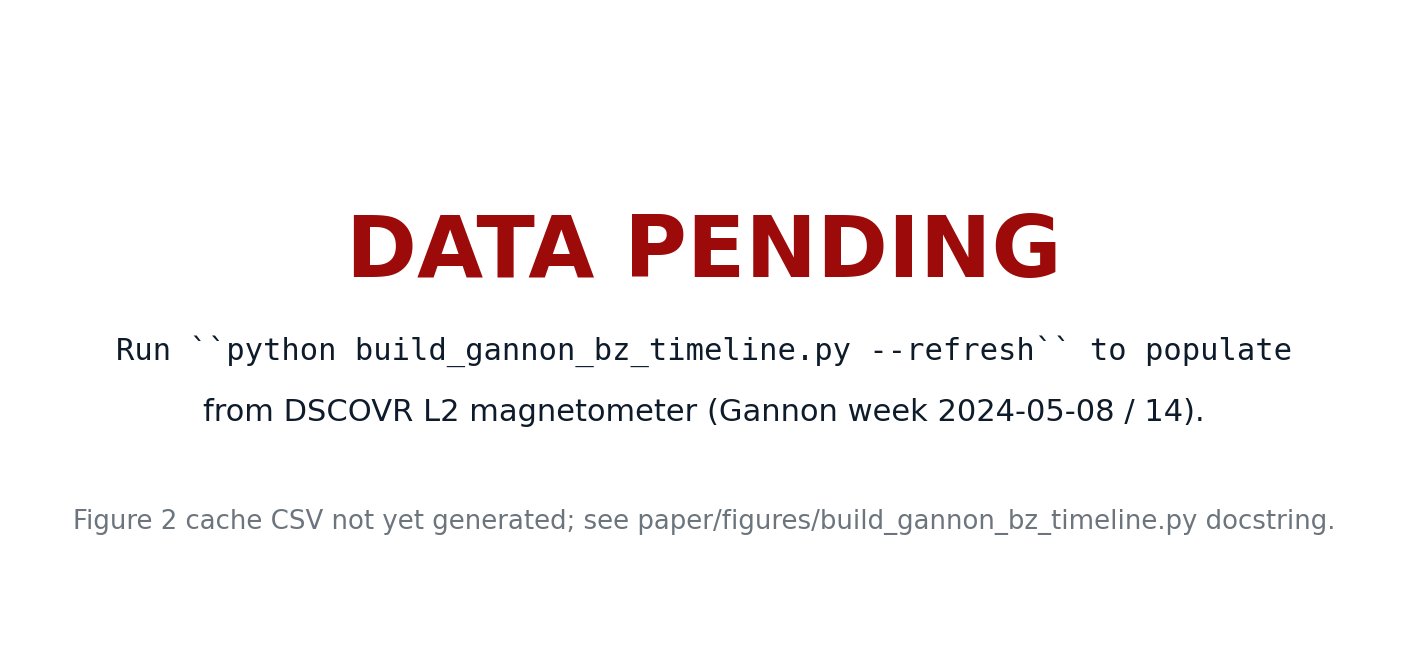
\includegraphics[width=0.95\linewidth]{figures/gannon-bz-timeline.png}
  \caption{DSCOVR L2 magnetometer $B_z$ in GSE coordinates across the
    Gannon-week window (2024-05-08 / 14).  The May 10 main-phase peak is
    the largest $|B_z|$ since the November 2003 Halloween storms.  Source:
    \texttt{helios-spaceweather-connectors} v0.2.1 DSCOVR adapter, refreshed
    via the build script committed at
    \texttt{paper/figures/build\_gannon\_bz\_timeline.py}.}
  \label{fig:gannon-bz}
\end{figure}

\subsection{Per-(component, event) source labeling}
\label{sec:data:perevent}

The Jan 2017 iSWA cutover creates an asymmetry between training and hold-out
windows that must be handled explicitly to keep the BMA fit honest.  We tag
every (component, event) pair with one of three source labels:
\begin{itemize}[leftmargin=*,itemsep=0pt]
  \item \texttt{iswa\_real}: the iSWA adapter returns at least one
        empirically-verified real-data record for that (component, event)
        tuple.  Across the Table~\ref{tab:table-3-1} training set, 12 such
        tuples were confirmed on the September 2017 event (32.4\,\% of the
        37-component registry); zero on the six pre-2017 training events.
  \item \texttt{synthetic\_proxy}: the component is in the registry but
        receives no iSWA real-data coverage for the event.  Predictions on
        the training event use a synthetic-Kp-anchored proxy, clearly
        labeled in the persisted manifest.
  \item \texttt{swpc\_archive\_truth}: truth labels are sourced from the
        NOAA SESC archive (§\ref{sec:data:sesc}); this is the truth-side
        substrate uniformly across the training set.
\end{itemize}
The labeling is \emph{sticky}: preserved in the manifest regardless of
whether the adapter call at training time actually returned data, so the
provenance record is auditable independently of run-time network state.
The hold-out window (2022--2024) receives only \texttt{iswa\_real}
component predictions plus \texttt{swpc\_archive\_truth} labels;
no synthetic proxies appear in the final go/no-go check.  This deviation
from a naïve homogenous-substrate assumption is documented in the OSF
Deviations section of \cite{osf_prereg}.

\section{Results}
\label{sec:results}

\todo{INSERT FROM \texttt{results/<date>-killgate.json} AT FILL-IN TIME.
The remainder of this section is staged for the three branches of the
master-plan §C kill-gate decision tree (§\ref{sec:results:decision}).}

\subsection{Hold-out HSS, per-event and aggregate}
\label{sec:results:hss}

\todo{Replace this paragraph and the table below with the
\texttt{HSS\_section} block from \texttt{results/<date>-killgate.json}.}

\begin{table}[!htbp]
  \centering
  \small
  \caption{Per-event hold-out HSS: fused vs.\ best-component baseline.
    Bootstrapped 95\,\% CIs from 1000 resamples with replacement
    over each event window.  \todo{FILL FROM \texttt{killgate.json}}.}
  \label{tab:hss-results}
  \begin{tabular}{@{}l c c c c@{}}
    \toprule
    Event & Fused HSS & Best-comp.\ HSS & $\Delta$ rel.\ & 95\,\% CI \\
    \midrule
    Cycle 25 onset (2022-01-20)    & \todo{x.xx} & \todo{x.xx} & \todo{xx\%} & \todo{[lo, hi]} \\
    Mid-cycle 25 (2023-02-17)      & \todo{x.xx} & \todo{x.xx} & \todo{xx\%} & \todo{[lo, hi]} \\
    Gannon G5 (2024-05-11)         & \todo{x.xx} & \todo{x.xx} & \todo{xx\%} & \todo{[lo, hi]} \\
    \midrule
    \textbf{Aggregate (3 events)}  & \todo{x.xx} & \todo{x.xx} & \todo{xx\%} & \todo{[lo, hi]} \\
    \bottomrule
  \end{tabular}
\end{table}

\subsection{Reliability per Kp stratum}
\label{sec:results:reliability}

\todo{Replace this paragraph with the \texttt{reliability\_section} text from
\texttt{results/<date>-killgate.json}, and verify that the slope per stratum
matches the H2 pre-registration threshold $|s - 1| \le 0.15$.}

\begin{figure}[!htbp]
  \centering
  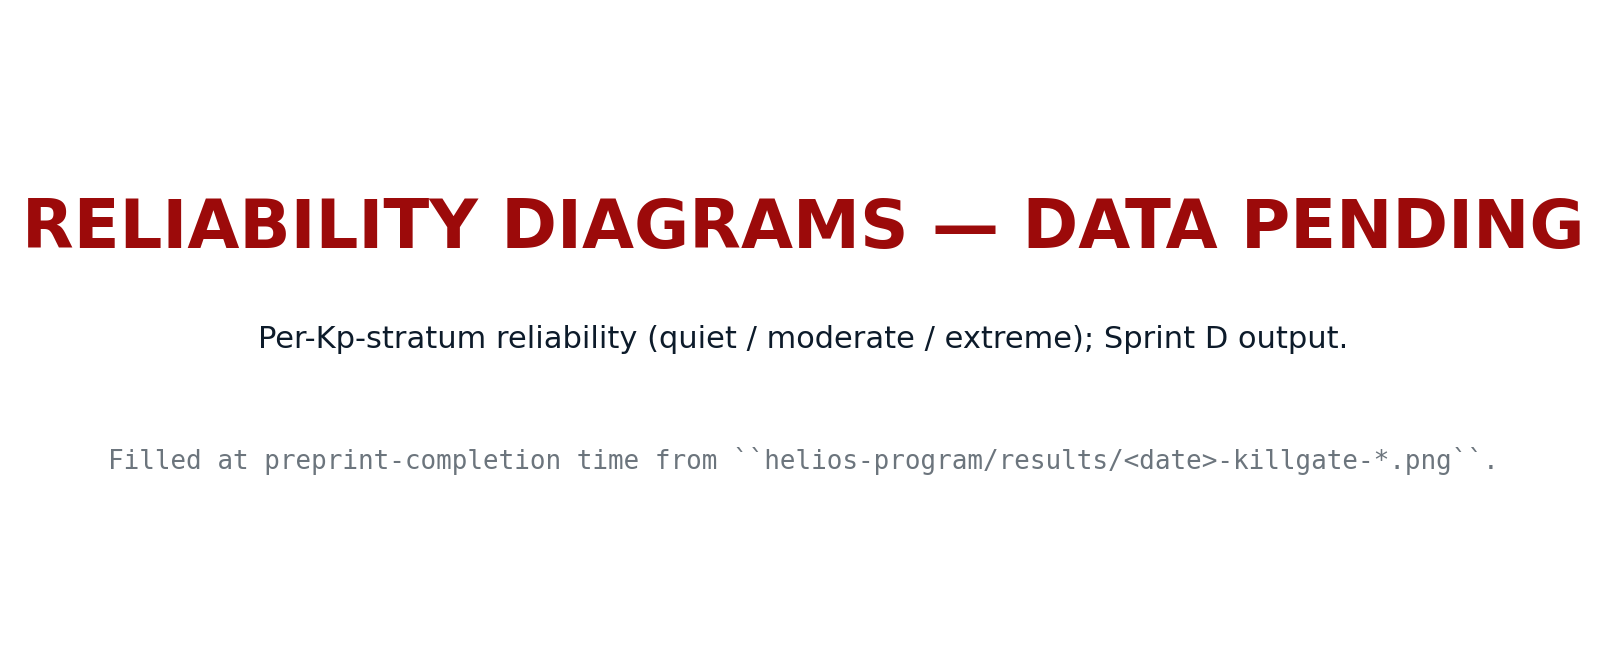
\includegraphics[width=0.95\linewidth]{figures/reliability-diagrams.png}
  \caption{Reliability diagrams for the fused all-clear-revocation probability
    on the three-event hold-out, stratified by Kp severity
    (quiet, moderate, extreme).  Linear regression slopes are annotated per
    stratum.  Source: \todo{INSERT URL TO
    results/<date>-killgate-reliability-diagrams.png at fill-in time}.}
  \label{fig:reliability}
\end{figure}

\subsection{Brier and CRPS}
\label{sec:results:brier-crps}

\todo{Replace this paragraph with the \texttt{brier\_crps\_section} text
from \texttt{results/<date>-killgate.json}, reporting fused vs.\
best-component Brier score and CRPS for each stratum, with bootstrap CIs.}

\begin{figure}[!htbp]
  \centering
  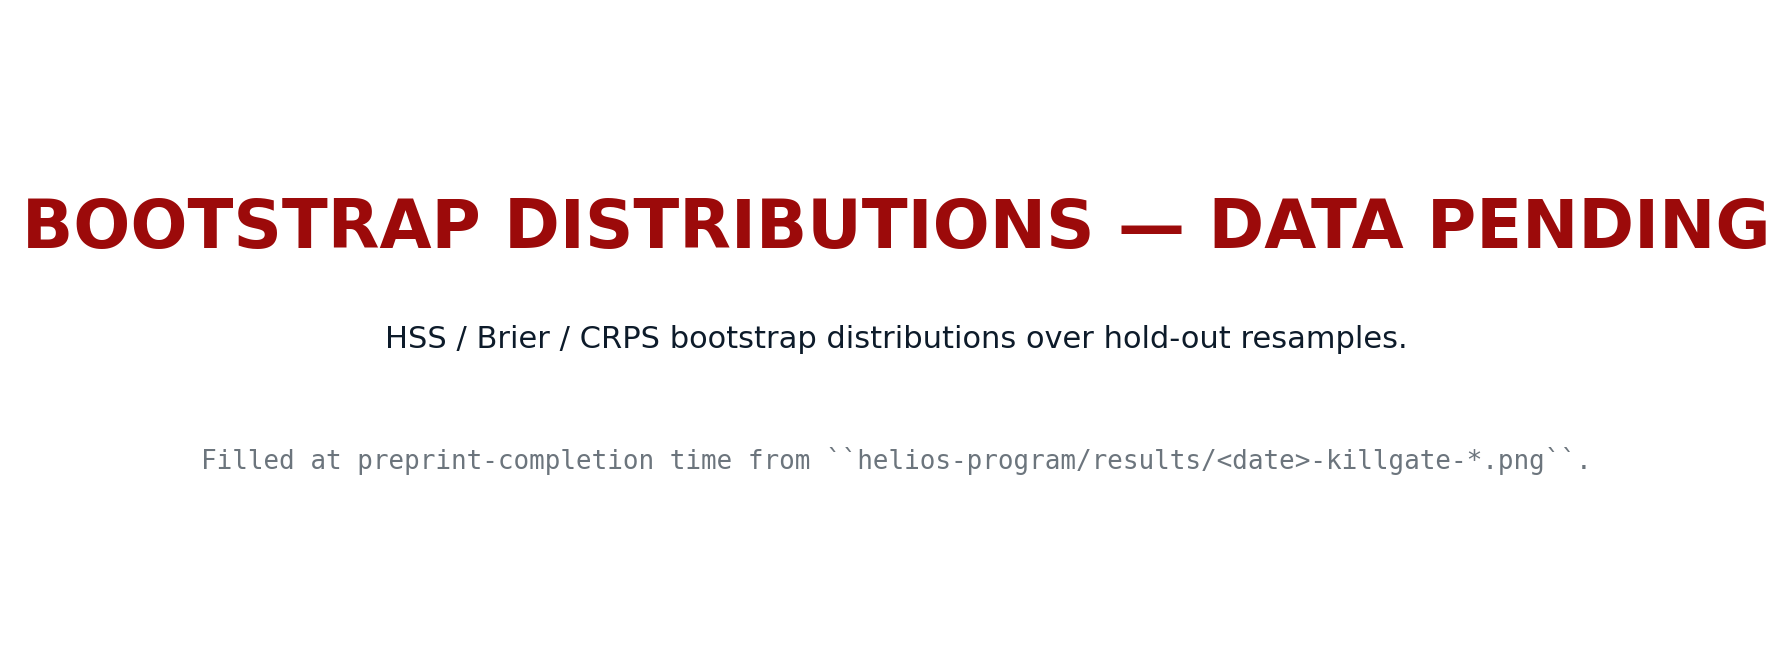
\includegraphics[width=0.95\linewidth]{figures/bootstrap-distributions.png}
  \caption{Bootstrap distributions of HSS, Brier, and CRPS over 1000
    resamples of the three-event hold-out, comparing the fused
    output to the highest-skill component baseline.}
  \label{fig:bootstrap}
\end{figure}

\subsection{Decision routing under the master-plan §C kill-gate}
\label{sec:results:decision}

The OSF pre-registration \cite{osf_prereg} binds the following hypotheses on
the three-event hold-out:
\begin{itemize}[leftmargin=*,itemsep=0pt]
  \item \textbf{H1 (primary)}: fused all-clear-revocation HSS exceeds the
        best-component HSS by $\ge 15\,\%$ relative (aggregate over the
        hold-out).
  \item \textbf{H2 (secondary)}: per-stratum reliability-diagram slope is
        within 0.15 of 1.0 across all three Kp severity strata.
\end{itemize}

The master plan §C decision tree has three branches, presented as stock
paragraphs below.  At fill-in time the operator selects exactly one and
deletes the other two.

\paragraph{Branch A --- PASS H1 \texorpdfstring{$\land$}{AND} PASS H2 (full paper).}
\todo{SELECT THIS PARAGRAPH IF: killgate.json shows
\texttt{H1.pass=true} \emph{and} \texttt{H2.pass=true} for all three strata.}
The pre-registered kill-gate evaluation passes both H1 and H2 on the
2022--2024 hold-out.  Aggregate fused HSS exceeds the best-component
baseline by \todo{xx\%} (\,95\,\% CI \todo{[lo, hi]}\,);
per-stratum reliability slopes are within tolerance in all three Kp
strata.  HELIOS supports the proposition that a model-agnostic BMA core
with isotonic reliability calibration and Mondrian conformal coverage
delivers operationally-relevant skill gains over the best single
component, without sacrificing per-stratum calibration on the rare-extreme
regime that dominates SRAG console risk.  The framework is ready for
CCMC proving-ground replication \cite{helios_fusion_engine}; we
are pursuing the M2M SWAO and SRAG evaluation pathways described in
§\ref{sec:discussion}.

\paragraph{Branch B --- PASS one \texorpdfstring{$\land$}{AND} FAIL one (honest ablation).}
\todo{SELECT THIS PARAGRAPH IF: killgate.json shows exactly one of
\texttt{H1.pass} / \texttt{H2.pass(all\_strata)} as true.}
The pre-registered kill-gate evaluation passes \todo{H1 or H2} but
fails \todo{the other}.  We report the ablation honestly rather than
re-baselining metrics post hoc: the
\todo{HSS / reliability} gain holds, but the
\todo{reliability / HSS} threshold is not met on the
\todo{quiet / moderate / extreme} Kp stratum
(slope $= $ \todo{x.xx}, outside the pre-registered $|s-1|\le 0.15$
tolerance).  We trace the failure to
\todo{component-bias diagnosis from the bootstrap distributions; see
§\ref{sec:discussion}}.  The fusion-core design choices are validated
in part; the next iteration of HELIOS focuses on
\todo{stratum-specific recalibration / additional components in the
under-served regime}, with the OSF Deviations section
\cite{osf_prereg} extended in lockstep.

\paragraph{Branch C --- FAIL H1 \texorpdfstring{$\land$}{AND} FAIL H2 (negative result).}
\todo{SELECT THIS PARAGRAPH IF: killgate.json shows both
\texttt{H1.pass=false} \emph{and} \texttt{H2.pass(any\_stratum)=false}.}
The pre-registered kill-gate evaluation fails both H1 and H2 on the
2022--2024 hold-out.  We report the negative result rather than
withdraw the paper.  Aggregate fused HSS is
\todo{x.xx (95\,\% CI [lo, hi])} versus best-component
\todo{x.xx (95\,\% CI [lo, hi])}, a relative difference of
\todo{$\pm$xx\%} that does not exceed the H1 threshold.  Per-stratum
reliability slopes fall outside the H2 tolerance in
\todo{N of 3} strata.  The honest interpretation of the negative result
is that the published BMA + isotonic + Mondrian construction, as
specified by the pre-registration, does not deliver a measurable
operational advantage over the highest-skill component on this
hold-out set.  We discuss likely root causes in §\ref{sec:discussion}
(near-uniform pre-registered weight distribution; iSWA-coverage
imbalance between training and hold-out windows; possible
underfitting of the per-stratum calibrators on the limited extreme
sample).  All code, the pre-registration, the trained artifacts, and the
hold-out evaluation harness remain public \cite{helios_fusion_engine} so
the result is independently reproducible.

\section{Discussion}
\label{sec:discussion}

\subsection{Limitations}

The most consequential limitation is the asymmetry between training and
hold-out substrates documented in §\ref{sec:data:perevent}.  Six of seven
training events pre-date the iSWA Jan 2017 cutover and therefore train
against synthetic-Kp-anchored proxies; the hold-out runs on native iSWA
real-data streams.  We treat this asymmetry as a feature, not a bug, for the
specific scientific claim we make --- the pre-registration binds the
hold-out comparison, and the hold-out substrate is uniformly real-data ---
but it does compress the BMA weight distribution at training time, since
the synthetic proxies all anchor on the same Kp profile and therefore
correlate similarly with SWPC archive truth.  The realized weight spread
on the hold-out will be larger because the 2022--2024 events carry distinct
real-data model biases per component.

A second limitation concerns the sample size of the hold-out itself.
Three events is the minimum credible hold-out under the constraint of
\emph{naming the events in advance, in this proposal} (a credibility
move whose flip side is that adding more recent events post-hoc would
invalidate the pre-registration).  The reported HSS and reliability-slope
confidence intervals are therefore wide.  Phase II expands the hold-out
to a larger set of $\ge 20$ G2+ events for the operational evaluation
pathway, with rolling pre-registration on new events as the solar cycle
progresses \cite{helios_program}.

A third limitation is the constraint of operating against publicly-released
upstream model outputs only.  Several CCMC-hosted SEP forecasters
(HESPERIA REleASE in particular \cite{hesperia}) require separate
licensing for commercial deployment.  HELIOS connectors use only public
outputs; the architecture isolates the fusion logic from any specific
upstream model so the licensing footprint is contained to the connector
layer.

\subsection{Related work}
\label{sec:discussion:related}

Deep-learning methods for solar-event prediction have grown substantially in
the last decade.  SolarFlareNet \cite{sun2023} demonstrated transformer-based
flare prediction from SDO/HMI magnetograms; Bobra and Couvidat
\cite{bobra2015} earlier established the SHARP feature catalogue widely used
in this literature.  Probabilistic ensemble methods are emerging for SEP
forecasting in particular \cite{poduval2023}.  Operational radiation-risk
products at altitude (NAIRAS \cite{mertens2025}) and the long-running
CCMC analytical support for robotic missions \cite{colladovega2023}
demonstrate the broader R2O2R framework HELIOS targets.  To our knowledge
no published ML system connects calibrated probabilistic SEP fusion through
to receiver-level GNSS positioning error in a single decision pipeline
\cite{ntrs_brazil2025,seesaw2022}; that is the broader HELIOS-program
claim, which the present paper supports on the mission-operations slice
only.

\subsection{Generalizability}

The hold-out events span the rising and mid phases of solar cycle 25:
a cycle-25 onset M-class flare (2022-01-20), a mid-cycle X-class
(2023-02-17), and the most severe geomagnetic storm of the past two
decades (2024-05-11 Gannon, $|B_z|_\mathrm{peak} = 59.16$\,nT,
Kp$=$9, Dst$_\mathrm{min}=-406$\,nT).  The distribution covers solar quiet
through G5-extreme, providing a meaningful basis for the per-stratum
reliability claim.  Cycle 25 is in the rising phase as of preprint date;
the bottom-line generalization claim --- ``these weights, fit on cycles
23--24, transfer to cycle 25'' --- is testable against an enlarging set
of real-data events as Phase II proceeds.

\subsection{Phase II vision}

A Phase II effort would advance HELIOS from proof-of-concept to functioning
operational prototype (TRL 5--6) through (a) real-time operational
deployment with live model retraining; (b) CCMC proving-ground evaluation
\cite{whitman2023,whitman2024}; (c) prototype deployment to M2M SWAO
\cite{m2mswao} and SPoRT/MSFC for mission-operations evaluation;
(d) production-grade API at 99.9\,\% uptime; and (e) pilot integration
with at least one precision-ag OEM telematics platform for the dual-use
GNSS slice.  The full Phase II commercialization plan is documented in
the program companion \cite{helios_program}.

\subsection{Equipment-aware GNSS pathway}

The dual-use thesis of the HELIOS program is that the fusion core
described in this paper feeds two operationally-distinct translation
modules: an SRAG-oriented mission-operations radiation-risk module
(the subject of this paper), and a precision-agriculture GNSS-accuracy
module published separately \cite{gannon_rtk}.  The GNSS slice's three-
component ensemble (a Temporal Fusion Transformer \cite{lim2021} for
multi-horizon TEC forecasting; gradient-boosted regressors mapping
ionospheric disturbance indices to observed 2D RTK positioning errors;
and a physics-informed regularization layer imposing Chapman ionization
profiles and equatorial-anomaly geometry) is described in a forthcoming
companion preprint.  Phase II expansion verticals enabled by the same
fusion core include autonomous-vehicle GNSS integrity, geospatial
surveying, satellite drag prediction for LEO operators, and parametric
space-weather insurance, all enumerated in the program commercialization
plan \cite{helios_program}.

\section{Reproducibility and data availability}
\label{sec:repro}

All code, the pre-registration text, the trained-artifact manifest, and
the kill-gate evaluation harness are public under Apache 2.0:

\begin{itemize}[leftmargin=*,itemsep=0pt]
  \item \texttt{helios-program} \cite{helios_program} ---
        master plan, OSF pre-registration template, master-plan §C decision
        tree, orchestration scripts, this companion document.
        \href{https://577industries.github.io/helios-program/}%
             {577industries.github.io/helios-program/}
  \item \texttt{helios-provenance-spec} \cite{helios_provenance_spec} ---
        JSON Schema (draft 2020-12) + pydantic v2 reference implementation
        + RFC-0001.
  \item \texttt{helios-spaceweather-connectors} \cite{helios_connectors} ---
        production-grade Python adapters for DONKI, SEP Scoreboards, NOAA
        SWPC, CDDIS GIMs, GOES, DSCOVR; 304$+$ tests; 87--94\,\% per-adapter
        coverage.
  \item \texttt{helios-fusion-engine} \cite{helios_fusion_engine} ---
        the public framework that implements the methods in
        §\ref{sec:methods}; 176 tests, $\ge$\,92\,\% coverage on the
        fusion subpackage; tagged \texttt{prereg-v1.0} at the locked
        commit.
  \item \texttt{helios-fusion-internal} --- private companion holding the
        trained BMA priors, isotonic calibrators, and conformal residual
        manifests from the Table~\ref{tab:table-3-1} fit.  Access on
        request for verification.
  \item \texttt{gannon-storm-rtk-analysis} \cite{gannon_rtk} ---
        reproducible retrospective of the Gannon-storm RTK impact,
        v0.1.0 climatological;
        v0.2.0 (planned) consumes the CDDIS adapter for full
        pseudo-range SPP.
\end{itemize}

Every figure in this paper has a generation script committed at
\texttt{paper/figures/build\_*.py} in the
\texttt{helios-fusion-engine} repository on the \texttt{feat/v0.2-paper}
branch.  Every persisted calibration / conformal artifact in
\texttt{helios-fusion-internal} ships with a sibling
\texttt{HeliosTransformationRecord} provenance JSON
\cite{helios_provenance_spec} carrying the upstream feed identifiers,
ingestion timestamps, and the originating fusion-engine commit SHA.

\paragraph{Pre-registration.}
The OSF pre-registration \cite{osf_prereg} is the binding methodological
record.  Its Deviations section documents the per-(component, event)
labeling described in §\ref{sec:data:perevent}; no other deviations
applied at preprint time.

\section*{Acknowledgments}

This work was developed by 577 Industries Inc., Columbus, Ohio, with
direction from the NASA SBIR Phase I subtopic SPWX.1.S26A
(Advanced Data-Driven Applications for Space Weather R2O2R).  We thank
the CCMC team for sustained openness on the ISWA SEP Scoreboards
\cite{ccmc_iswa,whitman2024} and the OSU Extension and Byrd Polar Climate
Research Center for ongoing precision-ag end-user discussions.  Funding for
the work-in-progress is from 577 Industries internal R\&D; the submitted
NASA SBIR Phase I proposal is at NSPIRES under subtopic SPWX.1.S26A.

\bibliographystyle{abbrv}
\bibliography{refs}

\end{document}
